
\section{Introduction}

The idea of \texttt{FLBEIA} comes from the similarities between the different models developed to perform bio-economic analysis in AZTI-Tecnalia. These models were pieces of code re-written in order to match with the specific case study or fishery. These pieces, in many cases, reflected exactly the same processes with similar dynamics that had to be slightly adapted to the different case studies. Therefore, in order to ease the job of the modelers, we decided to develop not a model but a framework in which a model is built. This model can be constructed combining already existing functions or developing new functions and combining them with existing ones. The choice of the kind of model to be used in a specific case study depends on the questions asked, which implies that not any model can be considered valid for all purposes.

Big advances have been done the last years in the field of bio-economic modelling with the development of models such as, Fishrent \citep{Salz2011}, Fcube \citep{Ulrich2011}, FcubeEcon \citep{Hoff2010} among others, and with the development of also some theoretical and partial assessments. However, until now there is no an universal model that can be applied to address all fishery management issues. Thus, we developed \texttt{FLBEIA} with the objective to integrate many of the models available in a common bio-economic impact assessment framework as a package of FLR \citep{Kell2007} in \citep{R2010}. \texttt{FLR} \citep{Kell2007} was built with the goal of developing a common framework to facilitate collaboration within and across disciplines (e.g. biological, ecological, statistical, mathematical, economic, and social) and, in particular, to ensure that new modelling methods and software are more easily validated and evaluated, and more widely available once developed.

The package \texttt{FLBEIA} contains the model called \texttt{FLBEIA}, a collection of functions and new \texttt{S4} classes developed to facilitate the simulation  of fishery systems in response to different types of management strategies. The model allows the evaluation of different management strategies, in a wide variety of case studies and scenarios, under Management Strategy Evaluation framework \citep{Butterworth1999, Butterworth2007, Delamare1998, Punt2007, Rademeyer2007}, and identifies the potential economic and biological consequences of a proposed policy action. 

The main characteristics of \texttt{FLBEIA} package are:

\begin{itemize}

	\item	It is coded in a generic, flexible and extensible way.
	\item Provides functions to condition the simulations, to run them and to analyze the results.

\end{itemize}	

In fact, a mayor effort has been set on the second functionality, namely the simulation model.

The main characteristics of the \texttt{FLBEIA} simulation model are:
\begin{itemize}
	
	\item The model is fully biological-economic coupled and provides fully integrated bio-economic assessment.
	\item The model deals with multi-species, multi-fleet and multi-\textit{metier} situations.
	\item The model can be run using seasonal steps (smaller or equal to one year).
	\item	It is generic, flexible and extensible.
  \item Uncertainty can be introduced in almost any of the parameters used.
	
\end{itemize}

A conceptual diagram of the model is  
shown in Figure~\ref{fig:MSE_diagram}. The simulation is divided in two main blocks:
the Operating Model (OM) and the Management Procedure Model (MPM). The OM is the part of the 
model that simulates the real dynamics of the fishery system and the MPM is the part of the model that simulates the whole management process. 

\begin{figure}[ht]
  \centering
    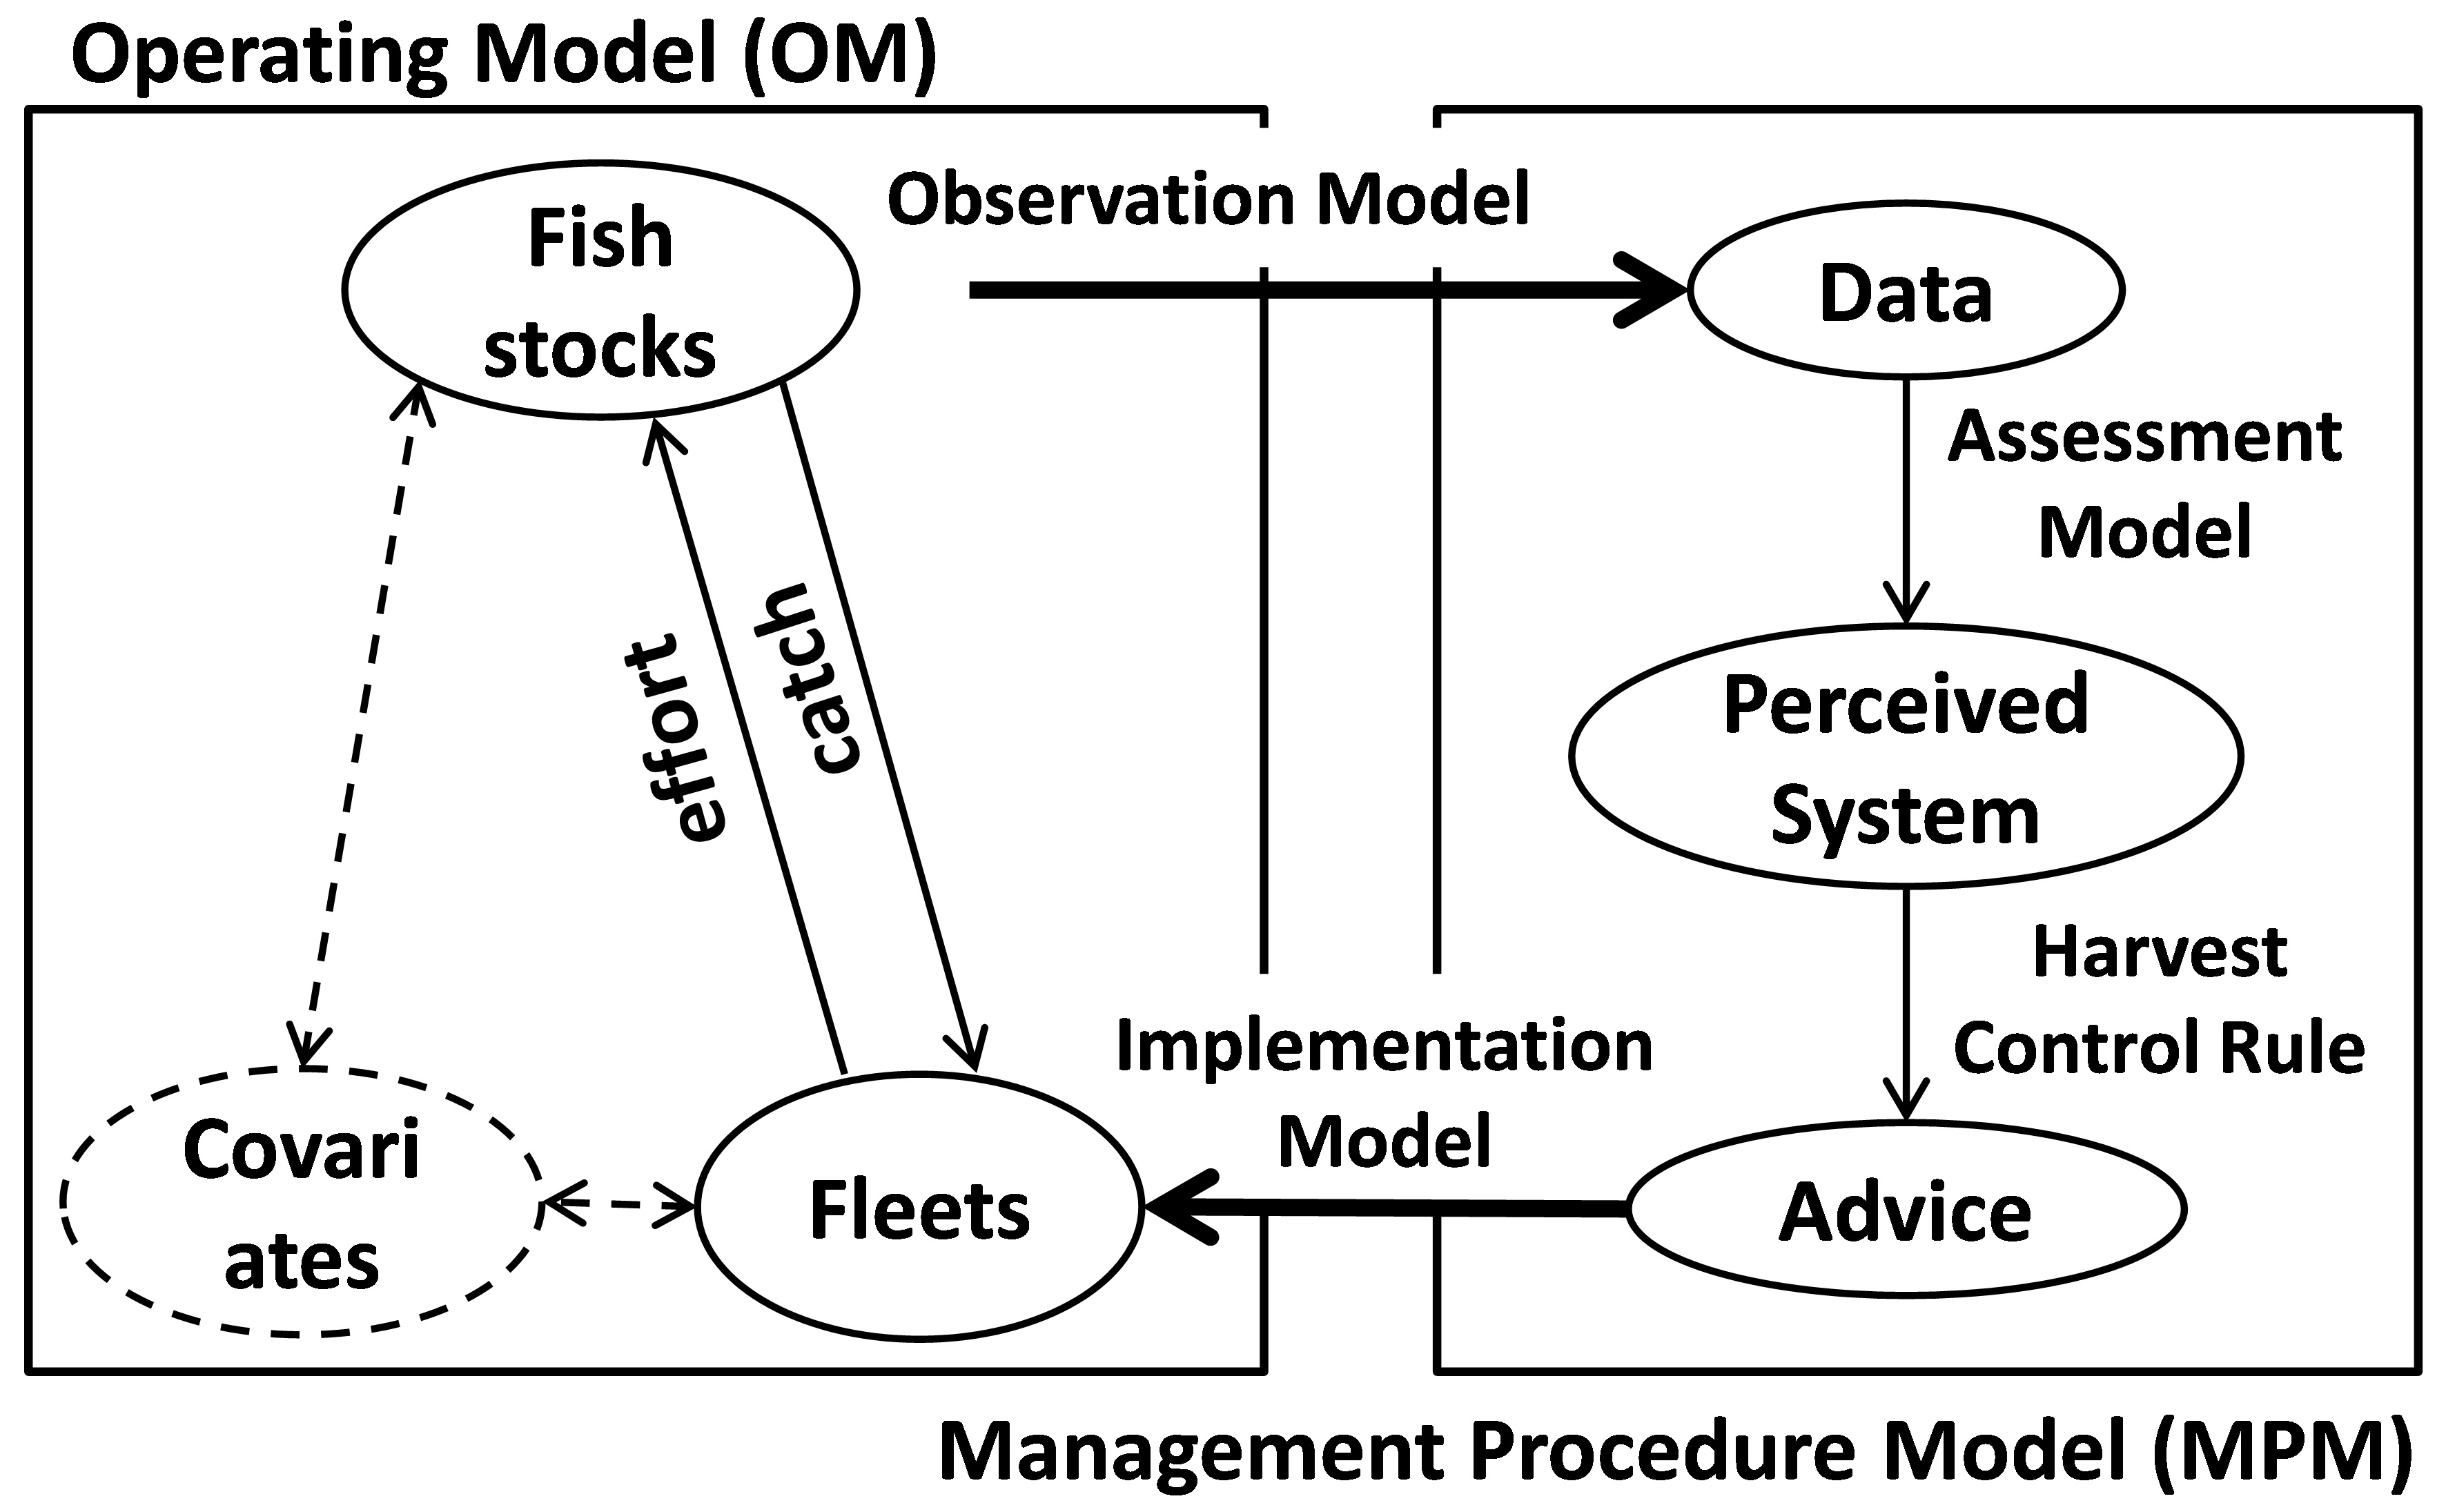
\includegraphics[width= 0.9\textwidth]{MSE_diagram}
  \caption{Conceptual representation of the main components modelled in FLBEIA. Source: \citep{Garcia2013}}
  \label{fig:MSE_diagram}
\end{figure}

The OM has three components that can interact among themselves:

\begin{enumerate}
	\item The biological populations or stocks.
  \item The fleets. 
  \item The covariates. They can be of any nature; environmental, economical or technical.
\end{enumerate}

The MPM has also three components:
\begin{enumerate}
	\item The data collected from the OM. 
  \item The observed population obtained through the application of a set of assessment models to the observed data. 
  \item The management advice obtained from the application of harvest control rules (HCR) to the observed populations.
\end{enumerate}
 

The model is built modularly with a top-down structure that has, at least, four levels:
 
\begin{enumerate}
	\item In the first level (top level), there is only one function, \texttt{FLBEIA} function. 
	It calls the functions on the second level in a determined order and it links the main components	(stocks, fleets, covariates, data, observed population and management advice) of the OM and MPM.
	
	\item The functions in the second level correspond with the generation of each of the components in the Figure~\ref{fig:MSE_diagram}. The OM components project the objects one season forward: \texttt{biols.om} projects the stocks, \texttt{fleets.om} projects the fleets and \texttt{covars.om} projects the covariates. The MPM components generate the objects necessary to produce the management advice, they generate the objects based on OM objects and they operate at most once a year: \texttt{observation.mp} generates the data, \texttt{assessment.mp} generates the observed population and \texttt{advice.mp} generates the management advice. They take the input objects and return only those related to the component they belong to.
			
	\item The functions in the third level define the specific dynamics of each component 
	and they are chosen by the user in each simulation. They are always called by a second level function and in some cases, a third level function also calls fourth level functions. For example a function that describes the dynamics of an age structured population can call a stock recruitment function. In this way, a function used	to describe age structured populations can be combined with different stock recruitment relationships.  
  
	\item The functions in the fourth level are called by functions in the third level and are used to model the most basic processes in the simulation. They are coded as a function and selected by the user because it could be interesting to use the same third level function together with different fourth level functions, as in the case of age structured population and stock recruitment functions.
	
	 \end{enumerate}
	 
This top down structure allows avoiding the classical structure of separated biological and economic (and social) modules (that could be integrated or not). Therefore, when the model is designed and the modeler takes the decision of including a particular characteristic, it does not make any difference if the characteristic is biological or economical, only matters at which level the characteristic is.

\texttt{FLBEIA} framework permits to incorporate new third and lower level functions or to modify them, while first and second level ones are fixed. Changing first or second level functions would imply a different approach, but the existing third and lower level functions would be useful.

In the next Sections \texttt{FLBEIA}'s conceptual model and its specifications are explained. Firstly, in Section~\ref{sec:FLBEIAconcept}, the conceptual model characterizes the main components as well as the feedbacks and loops among them. Secondly, in Section~\ref{sec:FLBEIArun}, it is explained how to run FLBEIA to perform MSE. Thirdly, in Section~\ref{sec:FLBEIAfun}, the model specification describes the components, the currently available functions by level, and how to use them within the \texttt{FLBEIA} package. Next, in Section~\ref{sec:FLBEIASmartCond}, a way to easily condition the model is presented. And finally, in Section~\ref{sec:FLBEIAoutput}, the \texttt{FLBEIA} function output is described.
